\documentclass{beamer}
\usepackage{amsmath}
\usepackage[utf8]{inputenc}
\usepackage{hyperref}
\usepackage{multicol}
\usepackage{hyperref}

\inputencoding{utf8}

\mode<presentation> {
    \usetheme{Madrid}
}

\usepackage{graphicx}
\usepackage{booktabs}

\title[Introducciòn]{Introducci\'on a las Ciencias de la Computaci\'on}
\author{Ernesto Rodriguez}
\institute{
    Universidad del Itsmo \\
    \medskip \textit{erodriguez@unis.edu.gt}
}

\date[\today]{}

\begin{document}

\begin{frame}
\titlepage
\end{frame}

\begin{frame}
\frametitle{¿En que consisten las ciencias de la computaci\'on?}
{\bf Ejemplo \#1:} Un programa que crea laberintos
\begin{itemize}
    \item{Todo laberinto debe poder resolverse}
    \item{Todo laberinto debe ser divertido
    \begin{itemize}
        \item{Las soluciones deben ser \emph{unicas}}
        \item{Todos los cuartos deben ser \emph{accesibles}}
    \end{itemize}
    }
\end{itemize}
¿Como lo construimos?
\end{frame}

\begin{frame}
\frametitle{Bueno, a hackear}
\begin{center}
    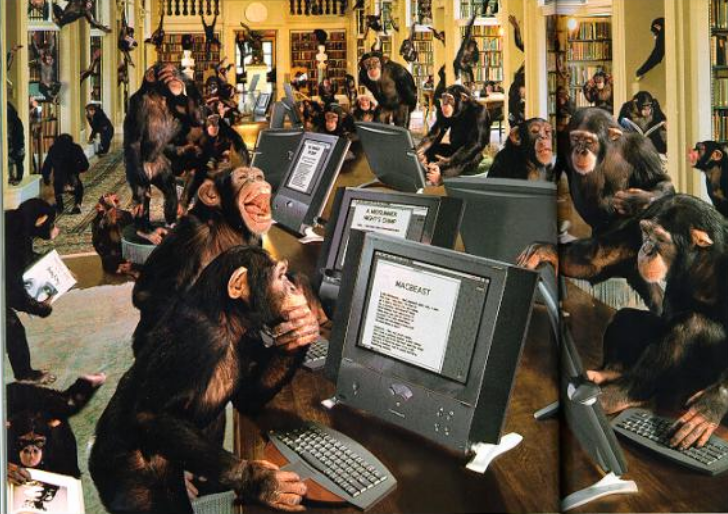
\includegraphics[width=10cm]{letshack.png}        
\end{center}
\end{frame}

\begin{frame}
\frametitle{Como razonar sobre el problema}
\begin{tabular}{ p{6cm} l }
{\begin{itemize}
    \item{Empezar con un laberinto completo}
    \item{Eliminar paredes al azar hasta tener un buen laberinto.}
    \item{A cada cuarto se le puede dar un nombre}
\end{itemize}} & \raisebox{-\totalheight}{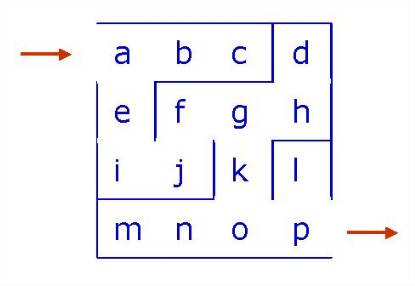
\includegraphics[width=4cm]{maze.png}} \\
\end{tabular}

{\bf Formulaci\'on Matematica:}
\begin{itemize}
    \item{Un conjunto de cuartos: $\{a,b,c,d,e,f,g,h,i,j,k,l,m,n,o,p\}$}
    \item{Parejas de cuartos que estan conectados. {\bf Ejemplo:} $\langle a,b \rangle$ o $\langle g, k\rangle$}
    \item{A esta estructura matematica se le conoce como un \emph{grafo}}
\end{itemize}

\end{frame}

\begin{frame}
\frametitle{¿Por que utilizamos la matematica?}
\begin{itemize}
    \item{¿Por que es util formular un problema como conjuntos y parejas?}
    \item{Las estructuras de datos se definen matematicamente}
    \item{La matematica nos ayuda a razonar acerca de la exactitud y eficiencia
    de nuestros algoritmos.}
    \item{Las estructuras matematicas nos ayudan a \emph{pensar} -- nos \emph{abstraen}
    de los detalles inecesarios para evitar ``hackear''}
\end{itemize}
\end{frame}

\begin{frame}
\frametitle{Laberintos como Grafos}
\begin{itemize}
    \item{{\bf Definici\'on:} Un grafo es un conjunto de \emph{nodos} y \emph{vertices} \--\--
    Son una de las estructuras de datos m\'as utilizadas en las CC}
    \item{{\bf Definici\'on:} Un \emph{laberinto} es un grafo con dos nodos especiales \--\--
    denominados como entrada y salida}
\end{itemize}
{\bf Interpretaci\'on:} Cada \emph{nodo} del grafo representa un cuarto. Un \emph{vertice}
$\langle a,b \rangle$ indica que el cuarto $a$ esta conectado con el cuarto $b$.
\begin{tabular}{c p{6cm}}
    \raisebox{-\totalheight}{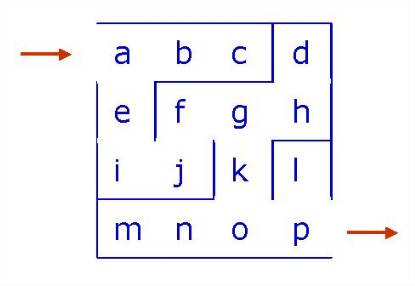
\includegraphics[width=5cm]{maze.png}} &
    $$
        \left\langle \left\{
            \begin{bmatrix}
                \langle a,e \rangle & \langle e, i\rangle & \langle i,j \rangle \\
                \langle f,j \rangle & \langle f,g \rangle & \langle g,h \rangle \\
                \langle d,h \rangle & \langle g,k \rangle & \langle a,b \rangle \\
                \langle m,n \rangle & \langle n,o \rangle & \langle b,c \rangle \\
                \langle k,o \rangle & \langle o,p \rangle & \langle l,p \rangle \\
            \end{bmatrix}
        \right\}, a, p \right\rangle
    $$ \\
\end{tabular}
\end{frame}

\begin{frame}
\frametitle{Laberintos como Grafos (visualizaci\'on)}
\begin{itemize}
    \item{Los grafos son objetos abstractos por lo cual es util una forma intuitiva de
    visualizarlos. Una opcion es un diagrama, donde los \emph{nodos} se visualizan como
    puntos y los \emph{vertices} como lineas.}
\end{itemize}
\begin{tabular}{p{6cm} c}
    $$
    \left\langle \left\{
        \begin{bmatrix}
            \langle a,e \rangle & \langle e, i\rangle & \langle i,j \rangle \\
            \langle f,j \rangle & \langle f,g \rangle & \langle g,h \rangle \\
            \langle d,h \rangle & \langle g,k \rangle & \langle a,b \rangle \\
            \langle m,n \rangle & \langle n,o \rangle & \langle b,c \rangle \\
            \langle k,o \rangle & \langle o,p \rangle & \langle l,p \rangle \\
        \end{bmatrix}
    \right\}, a, p \right\rangle
$$
&
\raisebox{-\totalheight}{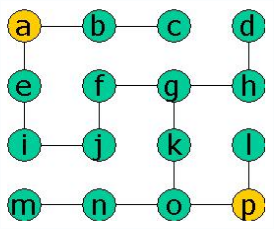
\includegraphics[width=4cm]{grafo.png}} \\
\end{tabular}
\\
Tomar en cuenta que la que el diagrama es una {\bf visualizaci\'on} del
grafo, no el grafo actual.
\end{frame}

\begin{frame}
\frametitle{Soluciones unicas}
\begin{tabular}{p{6cm} c}
\begin{itemize}
    \item{¿Que \emph{propiedad} debe tener un laberinto para que exista
    una soluci\'on?}
    \item{¿Que propiedad debe tener un laberinto para que la soluci\'on
    sea unica?}
\end{itemize} &
\raisebox{-\totalheight}{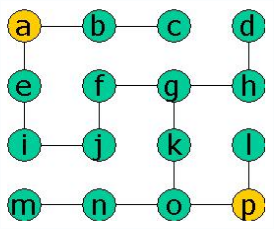
\includegraphics[width=4cm]{grafo.png}}
\end{tabular}
\end{frame}

\begin{frame}
    \frametitle{Soluciones unicas}
    \begin{tabular}{p{6cm} c}
    \begin{itemize}
        \item{¿Que \emph{propiedad} debe tener un laberinto para que exista
        una soluci\'on?
        \begin{itemize}
            \item{Debe existir un camino entre $a$ y $b$}
        \end{itemize}
        }
        \item{¿Que propiedad debe tener un laberinto para que la soluci\'on
        sea unica?
        \begin{itemize}
            \item{El grafo debe ser un \emph{arbol}}
        \end{itemize}
        }
    \end{itemize} &
    \raisebox{-\totalheight}{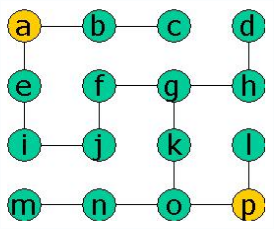
\includegraphics[width=4cm]{grafo.png}}
    \end{tabular}
\end{frame}

\begin{frame}
\frametitle{Laberintos como arboles}
\begin{tabular}{p{7cm} c}
\begin{itemize}
    \item{{\bf Definici\'on} Un \emph{arbol} es un grafo que:
    \begin{itemize}
        \item{Existe un unico \emph{nodo raiz}}
        \item{Cada nodo tiene un \emph{padre}}
    \end{itemize}
    }
\end{itemize}
\begin{itemize}
    \item{{\bf Definici\'on:} Un \emph{arbol abarcador} es un arbol que incluye todos los nodos.
    \begin{itemize}
        \item{¿Por que es importante tener un \emph{arbol abarcador}?}
    \end{itemize}
    }
\end{itemize}
&
\raisebox{-\totalheight}{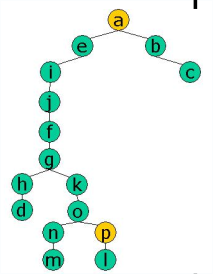
\includegraphics[height=5cm]{arbol.png}}
\end{tabular}
\end{frame}

\begin{frame}
    \frametitle{Laberintos como arboles}
    \begin{tabular}{p{7cm} c}
    \begin{itemize}
        \item{{\bf Definici\'on:} Un \emph{arbol} es un grafo que:
        \begin{itemize}
            \item{Existe un unico \emph{nodo raiz}}
            \item{Cada nodo tiene un \emph{padre}}
        \end{itemize}
        }
    \end{itemize}
    \begin{itemize}
        \item{{\bf Definici\'on:} Un \emph{arbol abarcador} es un arbol que incluye todos los nodos.
        \begin{itemize}
            \item{¿Por que es importante tener un \emph{arbol abarcador}?
            \begin{itemize}
                \item{Todos los cuartos se pueden alcanzar desde la raiz}
                \item{El arbol no tiene ciclos}
            \end{itemize}
            }
        \end{itemize}
        }
    \end{itemize}
    &
    \raisebox{-\totalheight}{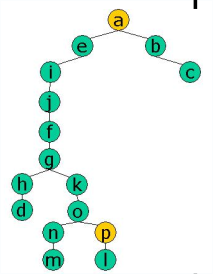
\includegraphics[height=5cm]{arbol.png}}
    \end{tabular}
\end{frame}

\begin{frame}
\frametitle{Algoritmo}
\begin{itemize}
\item{Ya que conocemos la estructura de datos, podemos considerar el algoritmo}
\item{{\bf Definici\'on:} Un \emph{algoritmo} es una serie de instrucciones para
controlar un proceso computable.}
\item{{\bf Ejemplo: } El algoritmo de Kruskal:
\begin{itemize}
    \item{Agregar una pareja al azar siempre y cuando no cree un ciclo}
    \item{Repetir hasta haber construido un \emph{arbol abarcador}}
\end{itemize}
}
\item{{\bf Ejemplo: } El algoritmo de \emph{Busqueda de Uniones}:
    \begin{itemize}
        \item{Colocar a los nodos para los que exista un camino en
        una misma \emph{clase de equivalencia}}
        \item{Antes de agregar un vertice $\langle x,y \rangle$, revisar
        que $x$ y $y$ no se encuentren en la misma \emph{clase de equivalencia}.}
    \end{itemize}
}
\end{itemize}
\end{frame}

\begin{frame}
\frametitle{¿Que tan rapido es nuestro algoritmo?}
\begin{itemize}
\item{¿Es rapido generar laberintos?
    \begin{itemize}
        \item{¿Que tan rapido se generan los laberintos?}
        \item{¿Que significa ``rapido''?}
    \end{itemize}
}
\item{Aparte de construir algoritmos, las ciencias de la computaci\'on tambien analizan
su rendimiento.}
\end{itemize}
\end{frame}

\begin{frame}
\frametitle{Rendimiento y escalabilidad}
\begin{itemize}
    \item{Supongamos que podemos escoger entre tres algoritmos.}
    \item{Dado un grafo con $n$ nodos, los algritmos toman $100n$, $7n^2$ y $2^n$ microsegundos ($\mu s$).}
\end{itemize}
\begin{center}
\begin{tabular}{|c|c|c|c|}
    \hline
    {\bf Tama\~no} & \multicolumn{3}{|c|}{\bf Rendimiento} \\
    \hline
    n & $100n$ & $7n^2$ & $2^n$ \\
    \hline
    1 & $100\mu s$ & $7\mu s$ & $2\mu s$ \\
    5 & $5ms$ & $175\mu s$ & $32\mu s$ \\
    10 & $1ms$ & $7ms$ & $1ms$ \\
    100 & $100ms$ & $7s$ & $10^{16}$ a\~nos \\
    1000 & $1s$ & $12m$ & - \\
    10000 & $10s$ & $20h$ & - \\
    \hline
\end{tabular}
\end{center}
\small{El tiempo ``-'' indica tiempos m\'as grandes que la edad del universo.}
\end{frame}

\end{document}